\documentclass{article}
\usepackage{amsmath}
\usepackage{tikz}

\begin{document}

\textbf{Problema:}
En una reunión clandestina se reunieron cierto número de mafiosos. Durante la noche de esa reunión, se realizó una redada y lograron capturar a uno de los contadores de los negocios de dicha reunión. El contador facilitó información para reducir su condena, a partir de dicha información los investigadores concluyeron que en la reunión había 83 personas y además, cada hombre conocía exactamente a nueve mujeres y cada mujer conocía exactamente a nueve hombres. Suponiendo que los investigadores no erraron sus conclusiones, determina si la información que facilitó el contador es verídica.

\bigskip

Para determinar si la información que proporcionó el contador es verídica, necesitamos desglosar la información y usar las relaciones que se nos han dado.

Supongamos que el número de hombres en la reunión es \( h \) y el número de mujeres es \( m \).

Sabemos que:
\begin{enumerate}
    \item \( h + m = 83 \) (la suma total de hombres y mujeres es 83)
\end{enumerate}

Dado que cada hombre conoce exactamente a 9 mujeres:
\begin{enumerate}
    \setcounter{enumi}{1}
    \item El total de conexiones entre hombres y mujeres es \( 9h \).
\end{enumerate}

Y como cada mujer conoce exactamente a 9 hombres:
\begin{enumerate}
    \setcounter{enumi}{2}
    \item El total de conexiones entre mujeres y hombres es también \( 9m \).
\end{enumerate}

Sin embargo, estas dos conexiones son equivalentes porque cuando un hombre conoce a una mujer, esa mujer conoce a ese hombre. Por lo tanto:
\[ 9h = 9m \]

De aquí podemos simplificar y obtener:
\[ h = m \]

Usando (1):
\[ h + h = 83 \]
Esto nos da:
\[ 2h = 83 \]

Lo cual es imposible porque 83 no es un número par. Por lo tanto, la información que el contador proporcionó no puede ser correcta.

\bigskip

\textbf{Visualización del Grafo:}

\begin{center}
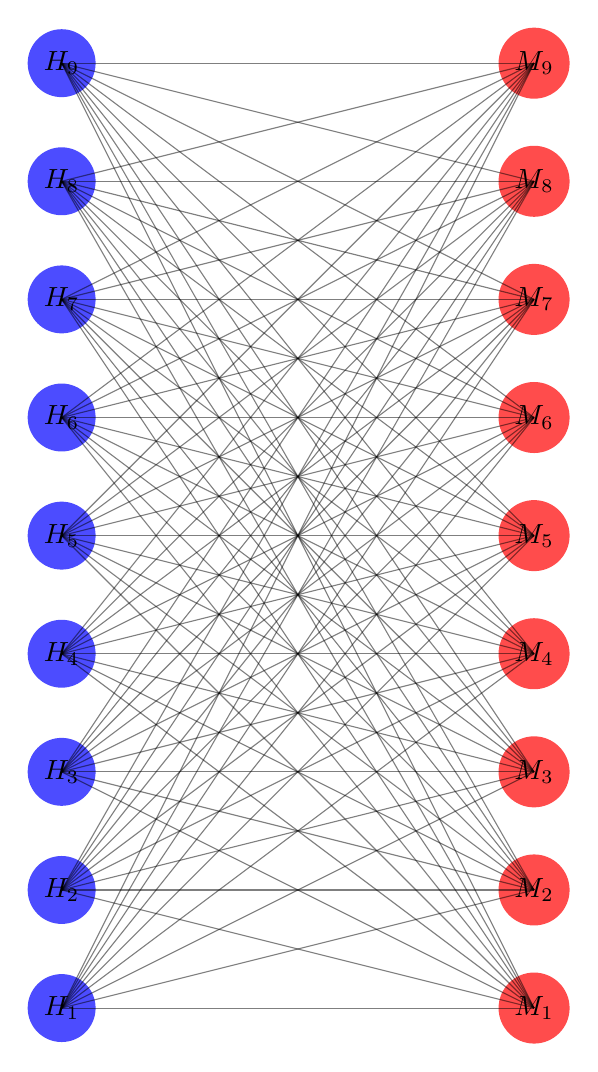
\begin{tikzpicture}[scale=1.5]
    % Hombres
    \foreach \i in {1,...,9} 
    {
        \node at (0,\i) [circle, fill=blue!70, minimum size=0.8cm] {$H_\i$};
    }

    % Mujeres
    \foreach \i in {1,...,9} 
    {
        \node at (4,\i) [circle, fill=red!70, minimum size=0.8cm] {$M_\i$};
    }

    % Conexiones
    \foreach \i in {1,...,9} 
    {
        \foreach \j in {1,...,9}
        {
            \draw[thin, opacity=0.5] (0,\i) -- (4,\j);
        }
    }
\end{tikzpicture}
\end{center}

\end{document}
